\definecolor{red}{rgb}{0.827,0.196,0.122}
\definecolor{orange}{rgb}{1.0,0.498,0.0}
\definecolor{olive}{rgb}{0.71,0.71,0.345}
\definecolor{green}{rgb}{0.118,0.490,0.216}
\definecolor{blue}{rgb}{0.447,0.624,0.812}

\chapter{Entwurf}
\label{chapter:design}
    Nachdem im vorangegangenem Kapitel die Anforderungen für das System spezifiziert wurden, soll in diesem Kapitel der Umsetzungsentwurf der verschiedenen Sichten dargestellt werden.
    Zunächst wird das dem System zugrundeliegende Datenmodell dargestellt.
    Darauffolgend wird das Design für die webbasierte Plattform erläutert.     
    
    \section{Datenmodell}
        \begin{figure}
            \centering
            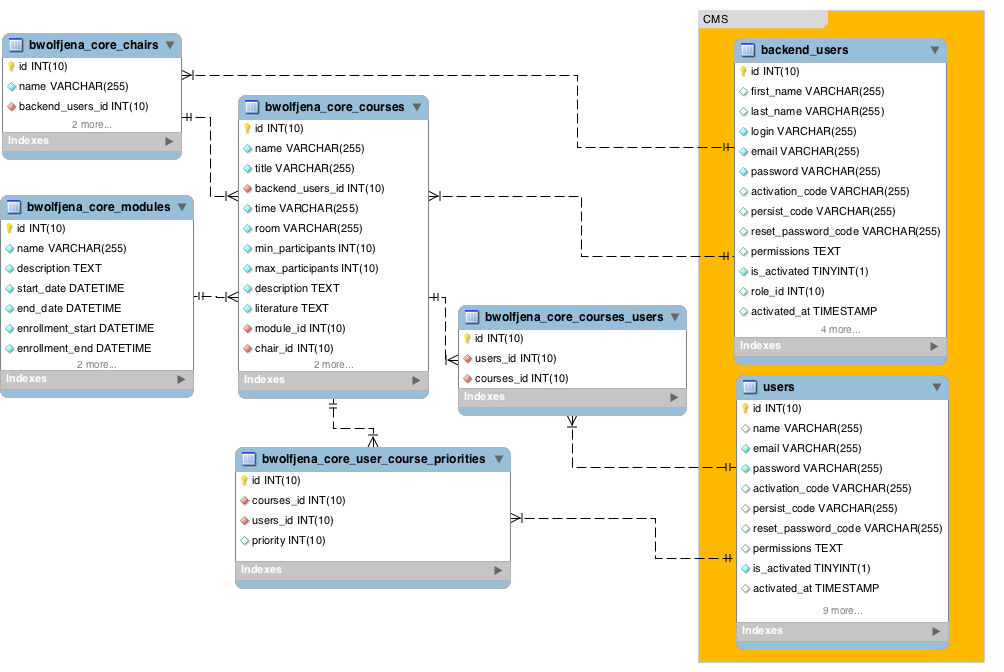
\includegraphics[width=1.0\textwidth]{./design/images/data-model.png}\par\vspace{1cm}
            \caption{Entwurf des Datenmodells. Farbcode für Spalten der Tabellen: Gelb Primärschlüssel, Rot Fremdschlüssel, Blau gewöhnliche Variable, Weiß nullable Variable}
            \label{fig:datamodel}
        \end{figure}
    
        Der Entwurf für das Datenmodell ist in Abbildung \ref{fig:datamodel} zu sehen.
        Es besteht aus sieben Tabellen.
        Die Tabelle \textit{bwolfjena\_core\_modules} beinhaltet die verschiedenen Empiriepraktika.
        Der Name Module für die Tabelle wurde gewählt, da das System bei Bedarf auch auf andere ausgewählte Module als das Empiriepraktikum erweitert werden kann.
        
        In der Tabelle \textit{bwolfjena\_core\_courses} sind die verschiedenen Kurse gespeichert.
        Ein Kurs gehört immer zu einem bestimmten Modul beziehungsweise einem Empiriepraktikum.
        Um das abzubilden, ist für jeden Kurs mittels eines Fremdschlüssels das Empiriepraktikum, zu dem er gehört, gespeichert.
        
        Ein Kurs wird immer von einem Lehrstuhl angeboten, die in der Tabelle \textit{bwolfjena\_core\_chairs} abgelegt sind.
        Auch auf diese Tabelle existiert wieder ein entsprechender Fremdschlüssel in \textit{bwolfjena\_core\_courses}. 
        
        Alle angemeldeten Studenten werden in der Tabelle \textit{users} gespeichert.
        Jeder der Studenten hat eine Präferenzliste.
        Die Einträge der Präferenzliste für jeden Studenten und jeden Kurs werden in Tabelle \textit{bwolfjena\_core\_priorities} gespeichert.
        Dementsprechend beinhaltet \textit{bwolfjena\_core\_priorities} Fremdschlüssel von \textit{users} und \textit{bwolfjena\_core\_courses}.
        
        In der Tabelle \textit{bwolfjena\_core\_users} ist abgelegt, welcher Student welchem Kurs zu geteilt wurde.
        Aus diesem Grund beinhaltet \textit{bwolfjena\_core\_users} Fremdschlüssel auf \textit{bwolfjena\_core\_courses} und \textit{users}. 
        
        Die letzte Tabelle \textit{backend\_users} beinhaltet die Backendbenutzer.
        Damit sind die Dozenten und Administratoren gemeint.
        In \textit{bwolfjena\_core\_courses} ist ein Fremdschlüssel für die Backendbenutzer gespeichert, um den Dozenten anzugeben, der den Kurs leitet.
        Auch die Tabelle \textit{bwolfjena\_core\_chairs} hat einen Fremdschlüssel zu der Tabelle \textit{backend\_users}, um den Lehrstuhlinhaber anzugeben.
        
        Neben den beschriebenen Fremdschlüsseln existieren für die Einträge in jeder Tabelle IDs als Primärschlüssel.
        Die weiteren Spalten der Tabellen sind entsprechend den Anforderung aus Kapitel \ref{chapter:requirements} gewählt.
        
        
        
    
    \section{Design}
        Für den Desing-Entwurf der Seite wurden Mock-Ups erstellt, die den groben Aufbau der Website mit den entsprechenden Funktionen zeigen. 
        Im folgenden werden diese Mock-Ups für das sogenannte Frontend, also aus Sicht der Studenten, und für das Backend, die Sicht der Dozenten beziehungsweise der Administratoren, vorgestellt.
        Dabei gilt der in Tabelle \ref{tab:Farbcode} angegebene Farbcode für die verschiedenen Elemente der Mock-Ups.
        \begin{table}
            \centering
            \begin{tabular}{l c| l}
                \cellcolor{red} & & Eingabefeld\\
                \cellcolor{orange} & & Button\\
                \cellcolor{olive} & & Drag\&Drop-Element\\
                \cellcolor{green} & & Textfeld\\
                \cellcolor{blue} & & Optisches Element
            \end{tabular}
            \caption{Farbcode der Mock-Ups}
            \label{tab:Farbcode}
        \end{table}
    
        \subsection{Frontend}
            Wie in Kapitel \ref{chapter:requirements} bereits ausgeführt, sollen die Studenten zunächst eine Registrierungs- bzw. Login-Oberfläche sehen.
            Jedoch sollen die verschiedenen Kurse auch ohne eine Anmeldung einsehbar sein.
            \begin{figure}[t]
            	\centering
            	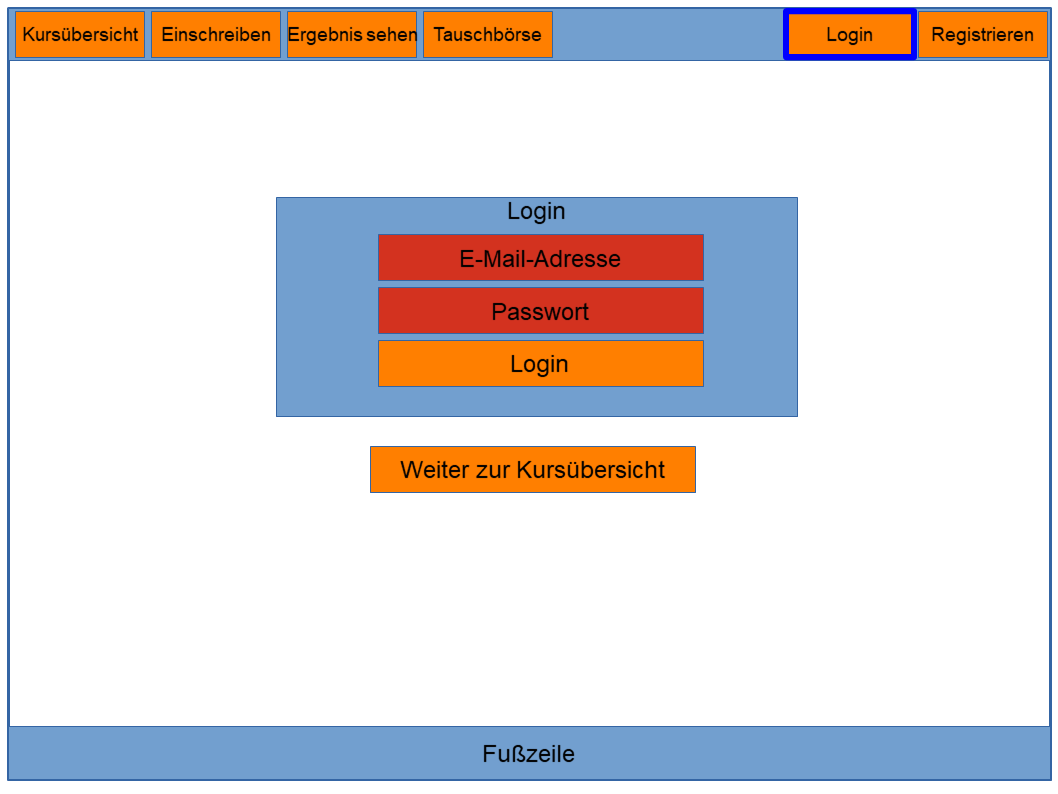
\includegraphics[width=0.7\textwidth]{./design/images/MockUpsFrontend/frontendLogin.png}
            	\caption{Entwurf für die Login-Oberfläche}
            	\label{mockupLoginFrontend}
            \end{figure}   
        
            In Abbildung \ref{mockupLoginFrontend} werden beide Anforderungen umgesetzt.
            Zum einen die Login-Oberfläche, in der in zwei Textfeldern Benutzername und Passwort für einen erfolgreichen Login eingetragen werden müssen, zum anderen die direkte Weiterleitung zur Kursübersicht als einfacher Knopf darunter.

            Die Kopfzeile umfasst einige Reiter.
            So kann mithilfe der Kopfzeile auf die verschiedenen Funktionen des Frontends gewechselt werden. 
            Dazu zählen die Kursübersicht, die Erstellung der Präferenzliste, das Einsehen der Verteilungsergebnisse, sowie das Tauschen von Kursen.
            Außerdem soll in der Kopfzeile ein Schalter zum Abmelden aus dem System bereitgestellt werden, sobald ein Benutzer die sich erfolgreich eingeloggt hat. 
%            Auch eine Anzeige, ab wann das Ende der Einschreibungs- und Tauschphase erreicht ist.
            Auf allen weiteren Seiten soll die Kopfzeile die gleiche Funktion und das gleiche Aussehen haben.
            Unter der Kopfzeile folgt eine textuelle Erklärung des Ablaufs des Empiriepraktikums und der für die Studenten relevanten Schritte, um sich erfolgreich für die Kurse einzuschreiben.
            Wie in Abbildung \ref{mockupCoursesFrontend} dargestellt, werden darunter die verschiedenen Kurse angezeigt, jeweils mit einer kurzen Beschreibung.
            Durch einen Klick auf ein Kursfeld, sollen sich die detaillierten Informationen zu dem Kurs einsehen lassen.
            Das Desing hierfür ist in Abbildung \ref{mockupDetailsFrontend} zu sehen und bedarf keiner weiteren Erläuterung.
            \begin{figure}[t]
            	\centering
            	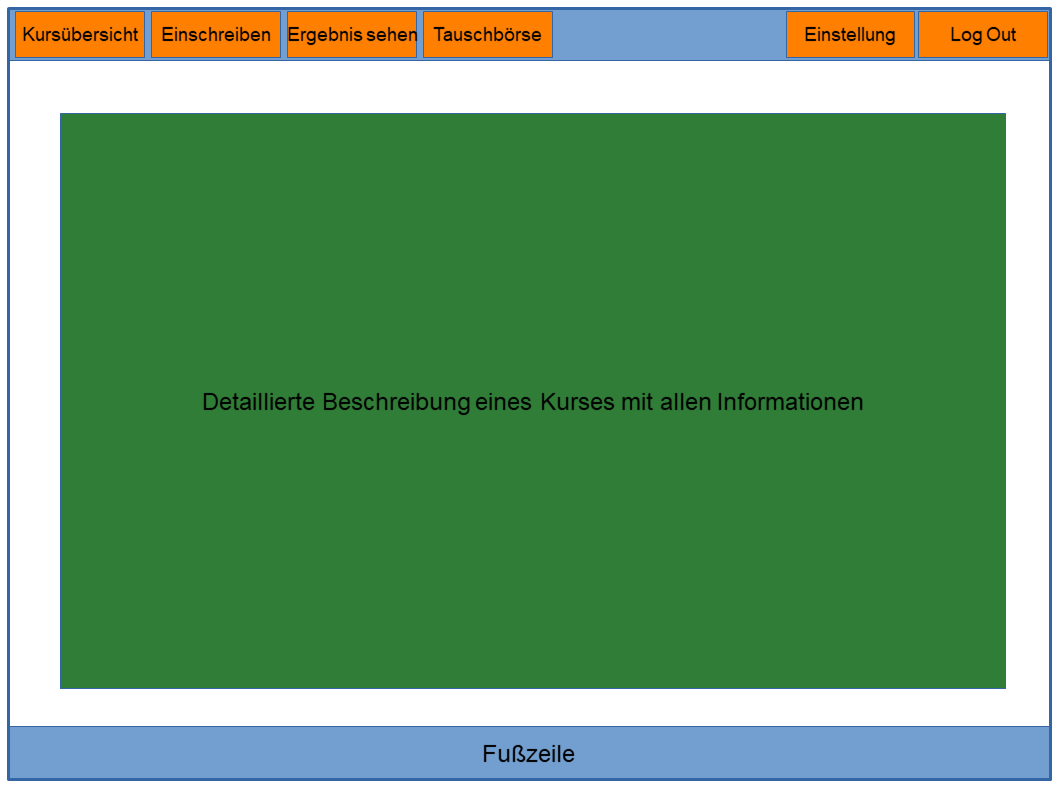
\includegraphics[width=0.7\textwidth]{./design/images/MockUpsFrontend/frontendCoursedetails.png}
            	\caption{Entwurf für die Kursdetails}
            	\label{mockupDetailsFrontend}
            \end{figure}
            Die Fußzeile soll weitere allgemeine Informationen bereitstellen, sofern diese von Nöten sein sollten, aber vor allem als optischer Abschluss der Seite dienen.
            \begin{figure}[t]
            	\centering
            	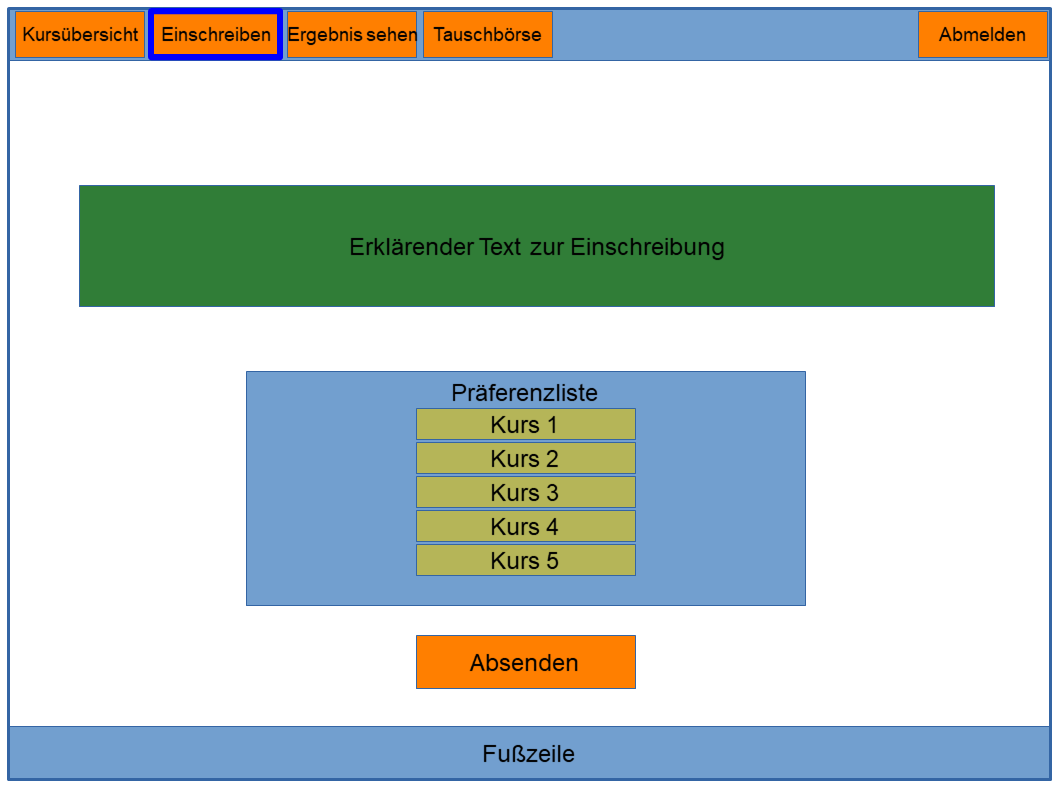
\includegraphics[width=0.7\textwidth]{./design/images/MockUpsFrontend/frontendPreferences.png}
            	\caption{Entwurf für die Einschreibungs-Oberfläche}
            	\label{mockupPreferencesFrontend}
            \end{figure}
            
            Die Seite für die Einschreibung in die Kurse soll wie in Abbildung \ref{mockupPreferencesFrontend} gestaltet sein.
            Wieder bilden Kopfzeile und Fußzeile den Rahmen der Seite.
            Unter der Kopfzeile befindet sich auch hier eine kurze Erklärung, wie man die Präferenzliste genau erstellt.
            Das Erstellen soll im Feld \textit{Präferenzliste} über ein ''Drag\&Drop''-System vorgenommen werden und über den Knopf \textit{Absenden} fixiert werden können.
            
            \begin{figure}[t]
                \centering
                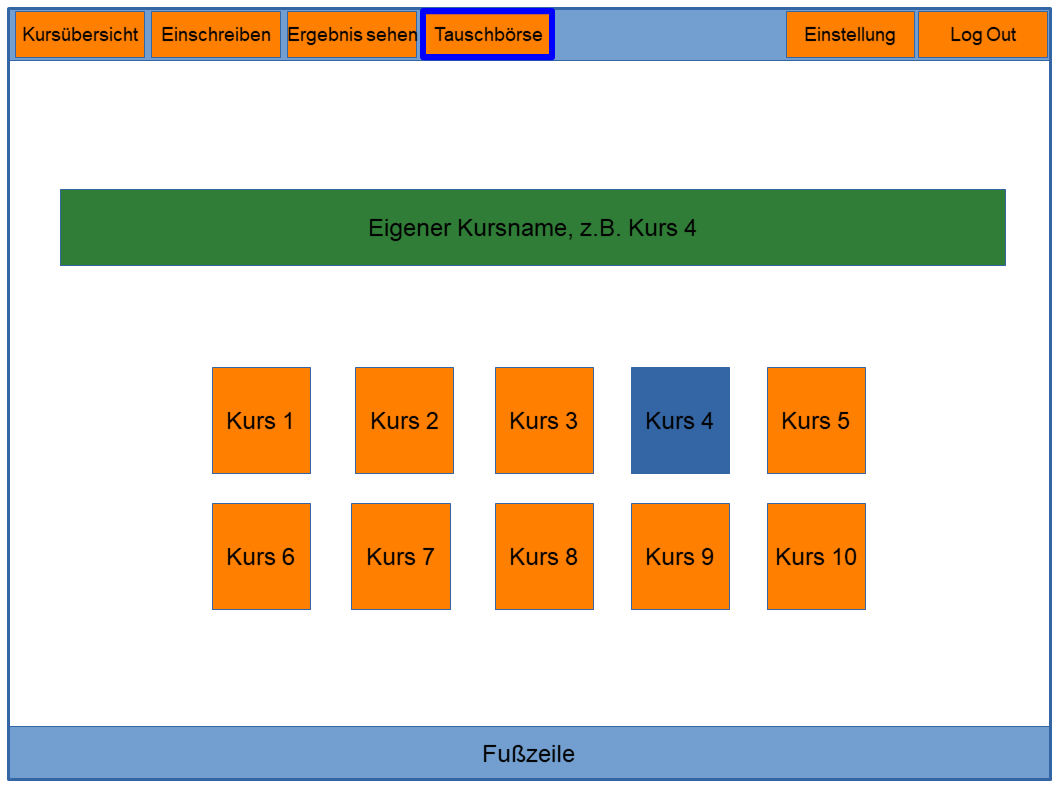
\includegraphics[width=0.7\textwidth]{./design/images/MockUpsFrontend/frontendSwap1.png}
                \caption{Entwurf für die Tauschauswahl}
                \label{mockupResultsFrontend}
            \end{figure}
        
            \begin{figure}[t]
                \centering
                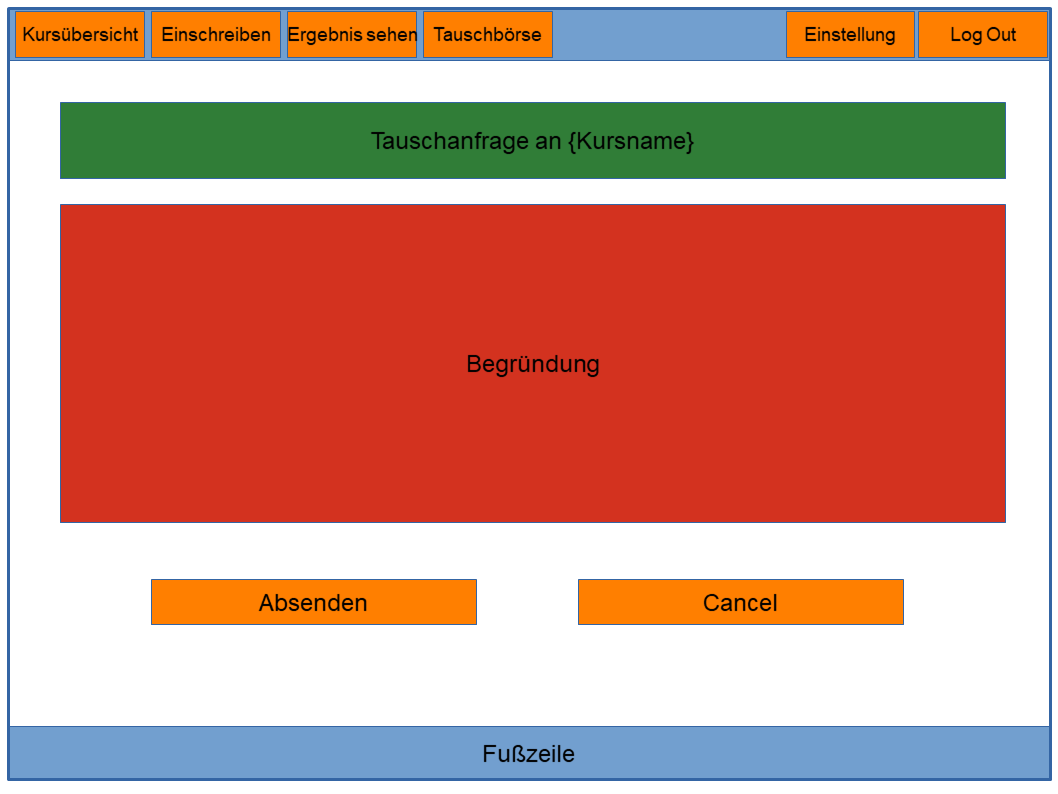
\includegraphics[width=0.7\textwidth]{./design/images/MockUpsFrontend/frontendSwap2.png}
                \caption{Entwurf für die Tauschanfrage}
                \label{mockupResultsFrontend}
            \end{figure}
            
    
        \subsection{Backend}
        	\subsubsection{Administratoren}
        	\subsubsection{Dozenten}